\documentclass[9pt,landscape]{article}
\usepackage{{./../static/style}}
\pdfinfo{
  /Title (PyAnsys Cheat Sheet)
  /Creator (TeX)
  /Producer (pdfTeX 1.40.0)
  /Author (Ansys)
  /Subject (PyAnsys)
  /Keywords (PyAnsys, Cheat sheet, template)}

\begin{document}
\raggedright
\footnotesize

% Add the title of cheat sheet here
% ----------------------------------------

\begin{center}
     \Huge{\textbf{PyFluent Cheat sheet}} \\
\end{center}
\begin{center}
     \Large{\textbf{Solver Settings Object Interface}} \\
     \small{\textbf{version:0.13 (stable)}} \\
\end{center}

\AddToShipoutPicture*
  {\put(670,577.5){
\includegraphics[height = 1.2cm]{ansys.png}}}
\AddToShipoutPictureBG*{
\includegraphics[width=\paperwidth]{bground.png}}
\vspace{-0.15cm}
\noindent\makebox[\linewidth]{\rule{\paperwidth}{2pt}}

\begin{multicols}{3}
\setlength{\premulticols}{1pt}
\setlength{\postmulticols}{1pt}
\setlength{\multicolsep}{1pt}
\setlength{\columnsep}{2pt}

% session starts here. 
% First colomn
% --------------------------------------------------------------------------------
\vfill
\section{
\includegraphics[height=\fontcharht\font`\S]{slash.png} Launch Fluent locally}
The following method is used to start Fluent from Python in gRPC mode.\\
This code starts Fluent in the background so that commands can be sent to Fluent from the Python interpreter.

\begin{lstlisting}[language=Python]
import ansys.fluent.core as pyfluent
solver = pyfluent.launch_fluent(mode = "solver", show_gui = True)
\end{lstlisting}

The solver object contains attributes such as \textbf{file}, \textbf{setup}, \textbf{solution}, and \textbf{results}, 
which are also instances of settings objects. 

% row 2 col 1
\section{
\includegraphics[height=\fontcharht\font`\S]{slash.png} Import mesh in launched session}

The following examples show how to read the available mesh file in Fluent Session.

\begin{lstlisting}[language=Python]
import_filename = 'example_file.msh.h5'
solver.file.read(file_type="case", file_name=import_filename)
\end{lstlisting}

There are other specific APIs available for reading case files and
reading case-data files. 

\begin{lstlisting}[language=Python]
# e.g., read_case(), read_case_data()

import_filename = 'example_file.cas.h5'
solver.file.read_case(file_type="case", file_name=import_filename)  
\end{lstlisting}


% row 3 col 1
\section{
\includegraphics[height=\fontcharht\font`\S]{slash.png} Enable heat transfer physics}

The following examples show how to enable heat transfer by activating the energy equation.

\begin{lstlisting}[language=Python]
solver.setup.models.energy.enabled = True
\end{lstlisting}

{
\includegraphics[height=\fontcharht\font`\S]{slash.png} Accessing the \textbf{object state} with using \textbf{pprint}

\begin{lstlisting}[language=Python]
>>> from pprint import pprint
>>> pprint(solver.setup.models.energy())
  {'enabled': True,
  'inlet_diffusion': True,
  'kinetic_energy': False,
  'pressure_work': False,
  'viscous_dissipation': False}  
\end{lstlisting}


% Second column
% --------------------------------------------------------------------------------
% row 1 col 2
\vfill
\section{
\includegraphics[height=\fontcharht\font`\S]{slash.png}  Define materials}
This example shows how you use Solver settings objects to define materials.
\begin{lstlisting}[language=Python]
solver.setup.materials.copy_database_material_by_name(type="fluid", name="water-liquid")
solver.setup.cell_zone_conditions.fluid["elbow-fluid"].material = "water-liquid"
\end{lstlisting} 

% row 2 col 2
\section{
\includegraphics[height=\fontcharht\font`\S]{slash.png}  Define boundary conditions}

The examples in this section show how you use Solver settings objects to define boundary conditions.

\begin{lstlisting}[language=Python]
solver.setup.boundary_conditions.velocity_inlet["cold-inlet"].vmag = {
    "option": "constant or expression",
    "constant": 0.4,
}
solver.setup.boundary_conditions.velocity_inlet[
    "cold-inlet"
].ke_spec = "Intensity and Hydraulic Diameter"
solver.setup.boundary_conditions.velocity_inlet["cold-inlet"].turb_intensity = 5
solver.setup.boundary_conditions.velocity_inlet[
    "cold-inlet"
].turb_hydraulic_diam = "4 [in]"
solver.setup.boundary_conditions.velocity_inlet["cold-inlet"].t = {
    "option": "constant or expression",
    "constant": 293.15,
}
\end{lstlisting} 

\vfill
{
\includegraphics[height=\fontcharht\font`\S]{slash.png}  Modify \textbf{cell zone} conditions} \\
The examples in this section show how you use Solver settings objects to modify \textbf{cell zone} conditions.
\begin{lstlisting}[language=Python]
# Enabling Laminar Zone

solver.setup.cell_zone_conditions.fluid["elbow-fluid"] = {"laminar": True}  
\end{lstlisting}
\vfill

% Third column
% --------------------------------------------------------------------------------
\vfill
% row 1 col 3
\section{
\includegraphics[height=\fontcharht\font`\S]{slash.png}  Apply solution settings}
PyFluent allows you to use Solver settings objects to apply
solution settings, initialize, and solve.

\begin{lstlisting}[language=Python]
solver.solution.initialization.hybrid_initialize()
solver.solution.run_calculation.iterate(number_of_iterations=150)
\end{lstlisting}

% row 2 col 3
\section{
\includegraphics[height=\fontcharht\font`\S]{slash.png}  Post-Processing}
PyFluent allows you to post-process data with \textbf{results} object. The following example shows you how to create and display contours on a plane.

\begin{lstlisting}[language=Python]
  solver.results.graphics.contour["contour"] = {}
  solver.results.graphics.contour["contour"].print_state()
  solver.results.graphics.contour["contour"].field = "temperature"
  solver.results.graphics.contour["contour"].surfaces_list = [
      "symmetry-xyplane",
  ]
\end{lstlisting}
\section{
\includegraphics[height=\fontcharht\font`\S]{slash.png}  Temperature Contour}
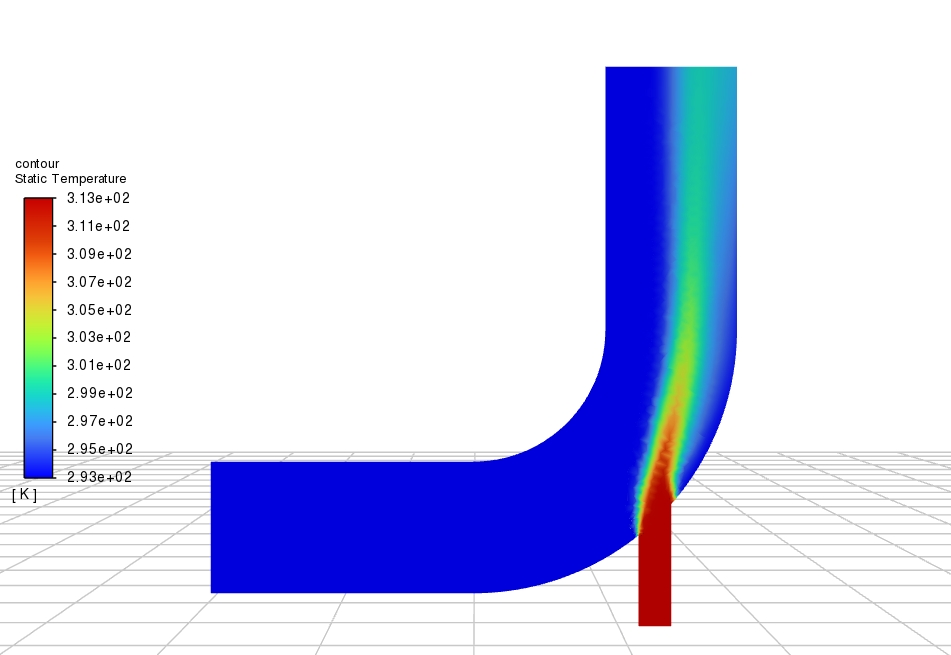
\includegraphics[scale=0.15]{mixing_elbow_pyfluent.jpg}
\centering


% Add subsection
% This section includes useful links to the documentation.
% Examples: installation, API reference, commands, examples.
% Replace 'name of link' with appropriate display text.

\subsection{References from PyAnsys Documentation}
\begin{itemize}
\item \href{https://fluent.docs.pyansys.com/release/0.13/getting_started/index.html}{\color{blue}{Getting Started}}  
\item \href{https://fluent.docs.pyansys.com/release/0.13/api/solver/settings.html#ref-settings}{\color{blue}{PyFluent Solver Settings Objects}}
\item \href{https://fluent.docs.pyansys.com/release/0.13/examples/index.html}{\color{blue}{PyFluent Examples}}
\end{itemize}
\end{multicols}

% Footer session of the latex with link to documentation and GitHub page
\vspace{-0.15cm}
\noindent\makebox[\linewidth]{\rule{\paperwidth}{4pt}}
\begin{center}
Getting Started with PyFluent 
\includegraphics[height=\fontcharht\font`\S]{slash.png} \href{https://github.com/ansys/pyfluent}{\color{blue}{PyFluent on GitHub}}} 
\includegraphics[height=\fontcharht\font`\S]{slash.png} Visit \code{\href{https://fluent.docs.pyansys.com/}}{\color{blue}{fluent.docs.pyansys.com}}
\end{center}
\end{document}